\documentclass[]{book}

%These tell TeX which packages to use.
\usepackage{array,epsfig}
\usepackage{amsmath}
\usepackage{amsfonts}
\usepackage{amssymb}
\usepackage{amsxtra}
\usepackage{amsthm}
\usepackage{mathrsfs}
\usepackage{color}
\usepackage{tikz}
\usepackage{enumerate}
\usepackage{hyperref}
\usepackage{chngcntr}
\usepackage{titlesec}
\usepackage{dsfont}



%Pagination stuff.
\setlength{\topmargin}{-.3 in}
\setlength{\oddsidemargin}{0in}
\setlength{\evensidemargin}{0in}
\setlength{\textheight}{9.in}
\setlength{\textwidth}{6.5in}
\pagestyle{empty}






\begin{document}

\begin{center}
{\Large Machine learning \hspace{0.5cm} HW 2}\\
\textbf{\small{Understanding Machine Learning: From Theory to Algorithms}[Exercises for chapters 3 and 5]}\\
\textbf{Mehrnaz jalili:400422061-
Arash Sajjadi:400422096}\\ %You should put your name here
\textit{Email: \href{mailto:Mehrnazjalili1991@gmail.com}{Mehrnazjalili1991@gmail.com}} 

\textit{Email: \href{mailto:arash.sajjadi@yahoo.com}{arash.sajjadi@yahoo.com}} 


Date: \today %You should write the date here.
\end{center}

\vspace{0.2 cm}

\section*{chapter 3}
\subsection*{Exercise 3.2:}

\begin{equation*}
\text{Preliminary assumptions}\left\{\begin{matrix}
 \mathcal{X} \longrightarrow & \text{Discrete} && \\ 
 \mathcal{H}=\left \{ h_z :z\in \mathcal{X} \right \} \cup \left \{ h^- \right \}&& h_z\left ( x \right )=\left\{\begin{matrix}
1 & x=z\\ 
0 & x\neq z
\end{matrix}\right.
\end{matrix}\right.
\end{equation*}

\subsubsection{3.2.1:}
Our algorithm will be that if $z$ is in our training set, this member will be labeled $+$, and all other members will be labeled $-$. If $z$ is not in our training set, all members must get a label. In both cases, the amount of training set's error is \textbf{zero}, so it is evident that our algorithm is an \textbf{ERM}.
\subsubsection{3.2.2:}
If there is no member with label $+$ in set $\mathcal{X}$ (whit respect to distribution $\mathcal{D}$), it is evident that our true label is a fixed function always returns $0$ (assign to each member of label $-$)
The question becomes a little more complicated when a member in $\mathcal{X}$ does not have a label $+$. In this case, two modes are possible. The first case is that we see this member in the training set, in which case, according to the algorithm presented in the previous section, we can claim to have achieved the true label. The second or rather the most challenging part of our problem is when the member with the label $+$ is inside  $\mathcal{X}$ but does not appear in the training set.In this we have:$\mathcal{D}(z)=\epsilon ,\mathcal{D}(x \neq z)=1-\epsilon $.\footnote{We can also show it by $\mathcal{D}(x^+)=\epsilon ,\mathcal{D}(x^-)=1-\epsilon $}.

%\begin{equation*}
%\mathbb{P}_{S \sim \mathcal{D}^m} \left [ S|_x,L_{\mathcal{D},f}>\epsilon \right ]<\delta \\
%\mathbb{P}\left [ x^+\notin S|_m \right ]=\left (1-\mathbb{P}(x^+)  \right )^m=\left (\mathbb{P}(x^-)  \right )^m=\\ \left ( 1-\epsilon \right )^m \leq e^{-\epsilon m}
%\end{equation*}

\begin{align*}
    \mathbb{P}_{S \sim \mathcal{D}^m} \left [ S|_x,L_{\mathcal{D},f}>\epsilon \right ]<\delta \\
\mathbb{P}\left [ x^+\notin S|_m \right ]= \\ \left (1-\mathbb{P}(x^+)  \right )^m=\left (\mathbb{P}(x^-)  \right )^m=\\ \left ( 1-\epsilon \right )^m \leq e^{-\epsilon m}
\end{align*}

At this stage we will easily have: $e^{-\epsilon m}\leq \delta \Rightarrow  m\geq \frac{\log\left ( \frac{1}{\delta} \right )}{\epsilon}$. Therfore, sample complexity is
bounded by

\begin{equation*}
    m_{\mathcal{H}}(\epsilon,\delta)\leq \left \lceil \frac{\log \left ( \frac{1}{\delta} \right )}{\epsilon} \right \rceil
\end{equation*}

\subsection*{Exercise 3.3:Concentric Circles}
\begin{equation*}
    \text{Preliminary assumptions}\left\{\begin{matrix}
\mathcal{X}=\mathbb{R}^2 & y=\left \{ 0,1 \right \}\\
\mathcal{H}=\left \{ h_r:r\in \mathbb{R}_+ \right \}  & h_r(x)=\mathds{1}_{[ \left \| x \right \| \leq r ]}
\end{matrix}\right.
\end{equation*}
Consider Algorithm $A$ in such a way that it returns the smallest circle that contains all the positive elements in our training set. Similarly to question number 3 in Chapter 2 of this book, this algorithm can be considered as an ERM.

We have to prove that $\mathcal{H}$ is PAC learnable.To solve the problem, we need a number of definitions, which we will introduce in this section.


\begin{itemize}
    \item \textbf{$R^*$} is a circle that represents our true label. But obviously, we do not have access to this circle because we do not have access to all the data in the universe of our data. So, and finding this circle is ideal for us. We also represent the radius of this circle with \textbf{$r^*$}. Also, the corresponding member of this circle in the set of hypotheses could be considered to be \textbf{$h^*$}.
    \item Consider $\hat{R}$ as the output of Algorithm $A$, which we talked about earlier. Similarly, $\hat{r}$ is the radius of the circle $\hat{R}$. $\hat{h}$ is also a member of our set of hypotheses that represents $\hat{R}$ for us.
    \footnote{$L_{S}(\hat{h}(x_{i\in [m]}))=0$}
    \item Perhaps the key to solving this problem depends on the definition of $R'$. We define $R'$ such that $r'\leq r^*$ and also for every $\epsilon,\delta \in (0,1)$, we have $\mathcal{D}_\mathcal{X} \left ( \left \{ x:r'\leq \left \| x \right \|\leq r^* \right \} \right )=\epsilon$. $r'$ and $h'$ are defined similarly to the previous items.
    %\item We can also define a set which is called $B$ such that $B=R^*-R'$.
    %\footnote{$B=R^*-R'$ also can be rewritten as $B=\left \{ x\in \mathbb{R}^2 : r'< \left \| x \right \| \leq r^*\right \}$. Since the probability of a curve is zero compared to a part of the plane, we can also here consider $B=\left \{ x\in \mathbb{R}^2 : r'\leq \left \| x \right \| \leq r^*\right \}$.}
\end{itemize}
It is clear that $\mathcal{D}(L_{\mathcal{D},f}(h_S)\geq \epsilon)$ is bounded above by the probability that no point $in$ S belongs to $(R^*-R')$. This probability of this event is bounded above by $(1-\epsilon)^m$. Having Taylor series, $(1-\epsilon)^m\leq e^{-\epsilon m}$


\begin{center}
    

\tikzset{every picture/.style={line width=0.75pt}} %set default line width to 0.75pt        

\begin{tikzpicture}[x=0.75pt,y=0.75pt,yscale=-1,xscale=1]
%uncomment if require: \path (0,300); %set diagram left start at 0, and has height of 300

%Shape: Circle [id:dp11502512002728116] 
\draw  [line width=1.5]  (205,154) .. controls (205,98.22) and (250.22,53) .. (306,53) .. controls (361.78,53) and (407,98.22) .. (407,154) .. controls (407,209.78) and (361.78,255) .. (306,255) .. controls (250.22,255) and (205,209.78) .. (205,154) -- cycle ;
%Shape: Circle [id:dp31846807923474274] 
\draw  [line width=0.75]  (244.7,154) .. controls (244.7,120.14) and (272.14,92.7) .. (306,92.7) .. controls (339.86,92.7) and (367.3,120.14) .. (367.3,154) .. controls (367.3,187.86) and (339.86,215.3) .. (306,215.3) .. controls (272.14,215.3) and (244.7,187.86) .. (244.7,154) -- cycle ;
%Shape: Circle [id:dp8681833990555992] 
\draw  [dash pattern={on 4.5pt off 4.5pt}] (228.85,154) .. controls (228.85,111.39) and (263.39,76.85) .. (306,76.85) .. controls (348.61,76.85) and (383.15,111.39) .. (383.15,154) .. controls (383.15,196.61) and (348.61,231.15) .. (306,231.15) .. controls (263.39,231.15) and (228.85,196.61) .. (228.85,154) -- cycle ;
%Straight Lines [id:da6909696580444573] 
\draw [line width=0.75]    (244.7,154) -- (306,154) ;
%Straight Lines [id:da03202867873850823] 
\draw  [dash pattern={on 4.5pt off 4.5pt}]  (306,154) -- (360,208) ;
%Straight Lines [id:da18877628222798148] 
\draw [line width=1.5]    (306,154) -- (336.67,57.33) ;

% Text Node
\draw (283,160) node [anchor=north west][inner sep=0.75pt]   [align=left] {+};
% Text Node
\draw (303,180) node [anchor=north west][inner sep=0.75pt]   [align=left] {+};
% Text Node
\draw (312,138) node [anchor=north west][inner sep=0.75pt]   [align=left] {+};
% Text Node
\draw (318,117) node [anchor=north west][inner sep=0.75pt]   [align=left] {+};
% Text Node
\draw (253,108) node [anchor=north west][inner sep=0.75pt]   [align=left] {+};
% Text Node
\draw (331,199) node [anchor=north west][inner sep=0.75pt]   [align=left] {+};
% Text Node
\draw (338,141) node [anchor=north west][inner sep=0.75pt]   [align=left] {+};
% Text Node
\draw (182,126) node [anchor=north west][inner sep=0.75pt]   [align=left] {\mbox{-}};
% Text Node
\draw (211,76) node [anchor=north west][inner sep=0.75pt]   [align=left] {\mbox{-}};
% Text Node
\draw (272,28) node [anchor=north west][inner sep=0.75pt]   [align=left] {\mbox{-}};
% Text Node
\draw (409,91) node [anchor=north west][inner sep=0.75pt]   [align=left] {\mbox{-}};
% Text Node
\draw (389,219) node [anchor=north west][inner sep=0.75pt]   [align=left] {\mbox{-}};
% Text Node
\draw (225,229) node [anchor=north west][inner sep=0.75pt]   [align=left] {\mbox{-}};
% Text Node
\draw (301,253) node [anchor=north west][inner sep=0.75pt]   [align=left] {\mbox{-}};
% Text Node
\draw (195,173) node [anchor=north west][inner sep=0.75pt]   [align=left] {\mbox{-}};
% Text Node
\draw (363,49) node [anchor=north west][inner sep=0.75pt]   [align=left] {\mbox{-}};
% Text Node
\draw (413,162) node [anchor=north west][inner sep=0.75pt]   [align=left] {\mbox{-}};
% Text Node
\draw (352,241) node [anchor=north west][inner sep=0.75pt]   [align=left] {\mbox{-}};
% Text Node
\draw (373,242) node [anchor=north west][inner sep=0.75pt]   [align=left] {\mbox{-}};
% Text Node
\draw (278,253) node [anchor=north west][inner sep=0.75pt]   [align=left] {\mbox{-}};
% Text Node
\draw (307,270) node [anchor=north west][inner sep=0.75pt]   [align=left] {\mbox{-}};
% Text Node
\draw (315,32) node [anchor=north west][inner sep=0.75pt]   [align=left] {\mbox{-}};
% Text Node
\draw (239,47) node [anchor=north west][inner sep=0.75pt]   [align=left] {\mbox{-}};
% Text Node
\draw (202,206) node [anchor=north west][inner sep=0.75pt]   [align=left] {\mbox{-}};
% Text Node
\draw (266.67,133.4) node [anchor=north west][inner sep=0.75pt]    {$\hat{r}$};
% Text Node
\draw (308,96.1) node [anchor=north west][inner sep=0.75pt]    {$r^{*}$};
% Text Node
\draw (340,167.73) node [anchor=north west][inner sep=0.75pt]    {$r'$};

%\node[above,font=\large\bfseries] at (current bounding box.north) {Some title};


\end{tikzpicture}

Our personal perception of this problem

\end{center}

\begin{equation*}
    \mathcal{D}(L_{\mathcal{D},f}(h_S)\geq \epsilon)=\mathcal{D}(S \cap \hat{R}=\varnothing )\overset{\text{i.i.d}}{=} (1-\epsilon)^m\leq e^{-\epsilon m} \leq \delta
\end{equation*}

Therfore, $\mathcal{H}$ is PAC learnable and the sample complexity is:
\begin{equation*}
    m_{\mathcal{H}}(\epsilon,\delta)\leq \left \lceil \frac{\log \left ( \frac{1}{\delta} \right )}{\epsilon} \right \rceil
\end{equation*}

\subsection*{Exercise 3.4:Boolean conjunctions}

Let's value $\mathcal{H}$ With the help of each other. There are three modes for each variable.


\begin{enumerate}
    \item $x_i$ exists in the multiplication function of variables.
    \item $\overline{x}_i$ exists in the multiplication function of variables.
    \item There is no combination of $x_i$ in our function.
\end{enumerate}

\begin{equation*}
    \left | \mathcal{H} \right |=3^d\Rightarrow \left | \mathcal{H} \right |:\text{finite}\Rightarrow \text{$\mathcal{H}$ is PAC learnable} \Rightarrow m_{\mathcal{H}}(\epsilon,\delta)\leq \left \lceil \frac{\log \left ( \frac{\left | \mathcal{H} \right |}{\delta} \right )}{\epsilon} \right \rceil
\end{equation*}
\begin{equation*}
    m_{\mathcal{H}}(\epsilon,\delta)\leq \left \lceil \frac{\log \left ( \frac{3^d}{\delta} \right )}{\epsilon} \right \rceil = \left \lceil \frac{d.\log \left ( 3 \right )-\log(\delta)}{\epsilon} \right \rceil
\end{equation*}
We couldn't answer this question entirely, but almost half of the questions have been answered.

\subsection*{Exercise 3.5:I.N.I.D}

\begin{equation*}
\text{Preliminary assumpti} \left\{\begin{matrix}
\mathcal{D}_m=\frac{\sum_{i=1}^{m}\mathcal{D}_i}{m}\\
\mathcal{X}\rightarrow \text{independent}
\\ S=\left \{ x_1,...,x_m \right \}\Rightarrow \left | S \right |=m 
\\ \text{realizability}\checkmark\hspace{1cm} f\in\mathcal{H},\epsilon \in (0,1)
\end{matrix}\right.
\end{equation*}
We have to show that $\mathbb{P}\left [ \exists h \in \mathcal{H}: L_{(\mathcal{D},f)}(h)>\epsilon \hspace{0.2cm}\text{and}\hspace{0.2cm} L_{(S,f)(h)=0)} \right ] \leq \left | \mathcal{H} \right |e^{-\epsilon m}$
\begin{equation*}
    \underset{S\sim\prod_{i=1}^{m}\mathcal{D}_i}{\mathbb{P}}[L_{S,f}(h)=0]\underset{\text{expand}}{=}\prod_{i=1}^{m}\underset{A_i}{\underbrace{\underset{x\sim \mathcal{D}_i}{\mathbb{P}}\left [ f(x)=h(x) \right ]}}=\prod_{i=1}^{m}A_i
\end{equation*}
According to the question form's hint, we can convert this expression into a summation as follows.
\begin{equation*}
    \prod_{i=1}^{m}A_i=\left (\left ( \prod_{i=1}^{m}A_i \right )^{\frac{1}{m}}  \right )^m\leq \left ( \frac{\sum_{i=1}^{m}A_i}{m} \right )^m\leq (1-\epsilon)^m\leq e^{-\epsilon m}
\end{equation*}
It is clear that the members of our set of hypotheses that $L_{(\mathcal{D},f)}(h)>\epsilon$ are less than $|H|$.  Therefore, up to $|H|$ we have to check the probability of $L_{S,f)}(h)=0$ on the members of $H$ that$L_{(\mathcal{D},f)}(h)>\epsilon$. Therefore
\begin{equation*}
    \mathbb{P}\left [ \exists h \in \mathcal{H}: L_{(\mathcal{D},f)}(h)>\epsilon \hspace{0.2cm}\text{and}\hspace{0.2cm} L_{(S,f)(h)=0)} \right ] \leq \left | \mathcal{H} \right |e^{-\epsilon m}
\end{equation*}

\subsection*{Exercise 3.6:}
\begin{equation*}
\begin{matrix}
\mathcal{D}^m\left ( S|_x:L_{D}(h_S)>\underset{h\in \mathcal{H}}{\min}L_{D}(h)>\epsilon \right )<\delta &  \text{and} \hspace{1cm} \exists A(S)\in \mathcal{H} \: \text{s.t} \hspace{0.1cm} L_{\mathcal{D},f}(A(S))=0 \: \: \text{(assume realizability)}    \\ 
\Rightarrow \forall m>m_\mathcal{H}(\epsilon,\delta):\underset{h\in \mathcal{H}}{\min}L_{D}(h)=0 & \Rightarrow  \mathcal{D}^m_\mathcal{X}\left ( \left \{ S|_x \::\,L_{\mathcal{D},f}(h)<\epsilon \right \} \right )<\delta \\
\end{matrix}
\end{equation*}

$\Rightarrow$ $A$ is a successful PAC learner of $\mathcal{H}$ and $\mathcal{H}$ is PAC learnable.

\subsection*{Exercise 3.7:The Bayes optimal predictor}
Let, $x\in \mathcal{X}, c:\text{conditional probability of a positive label
given }x$.
\begin{align*}
    \mathbb{P}\left [ f_\mathcal{D}X\neq y|X=x) \right ]=\mathds{1}_{c_x \geq 0.5}.\mathbb{P}\left [ Y=0|X=x \right ]+\mathds{1}_{c_x < 0.5}.\mathbb{P}\left [ Y=1|X=x \right ] \\
    =\mathds{1}_{c_x \geq 0.5}.(1-c_x)+\mathds{1}_{c_x < 0.5}.c_x=\min\{c_x,1-c_x\}
\end{align*}
Therefore, it can be calculated that 

\begin{align*}
    \mathbb{P}[g(X)\neq Y|X=x]=\mathbb{P}[g(X)=0|X=x].\mathbb{P}[Y=1|X=x]+ \mathbb{P}[g(X)=1|X=x].\mathbb{P}[Y=0|X=x]
\\
=\mathbb{P}[g(X)=0|X=x].c_x+ \mathbb{P}[g(X)=1|X=x].(1-c_x) \\
\geq \mathbb{P}[g(X)=0|X=x].\min\{c_x,1-c_x\}+ \mathbb{P}[g(X)=1|X=x].\min\{c_x,1-c_x\}
\end{align*}
It can be calculated that

\begin{align*}
    L_{\mathcal{D}}(f_\mathcal{D})=\mathbb{E}_{(x,y)\sim \mathcal{D}}[\mathds{1} _{[f_\mathcal{D}(x)\neq y]}] \\
=\mathbb{E}_{x\sim \mathcal{D}_X}\left [ \mathbb{E}_{y\sim \mathcal{D}_Y[\mathds{1} _{f_\mathcal{D}(x)\neq y}|X=x]} \right ]
\\ =\mathbb{E}_{x\sim {\mathcal{D}_x}}[c_x]
\\ \leq\mathbb{E}_{x\sim \mathcal{D}_X}\left [ \mathbb{E}_{y \sim \mathcal{D}_Y|x} [\mathds{1} _{[g(x)\neq y]|X=x}]=L_\mathcal{D} (g) \right ] 
\end{align*}

\subsection*{Exercise 5.2:}
\begin{enumerate}
    \item In general, the fewer features we have, the easier it is to solve the problem. The answer to the problem is probably more linear, and as a result, we will not have the problem of computation and also computational speed. On the other hand, the more data there is, the decrease our error. The problem becomes more difficult. Also, our answer to the functional problem is more complex.
    \item 
    \begin{equation*}
        \mathcal{H}_5\supseteq  \mathcal{H}_2 \hspace{1.5cm} e_{\text{AP}}\left ( \mathcal{H}_5 \right )\leq e_{\text{AP}}\left ( \mathcal{H}_2 \right )\hspace{1.5cm} \text{Complexity of }\mathcal{H}_5 \geq  \text{Complexity of }\mathcal{H}_2
    \end{equation*}
    Therefore, if the size of our training data set is small, work on two-dimensional data is recommended.
\end{enumerate}




\end{document}


